% section
\section*{Appendix} \label{section::appendix}
 % subsection
 \subsection*{Code structure}
  \begin{figure}[H]
   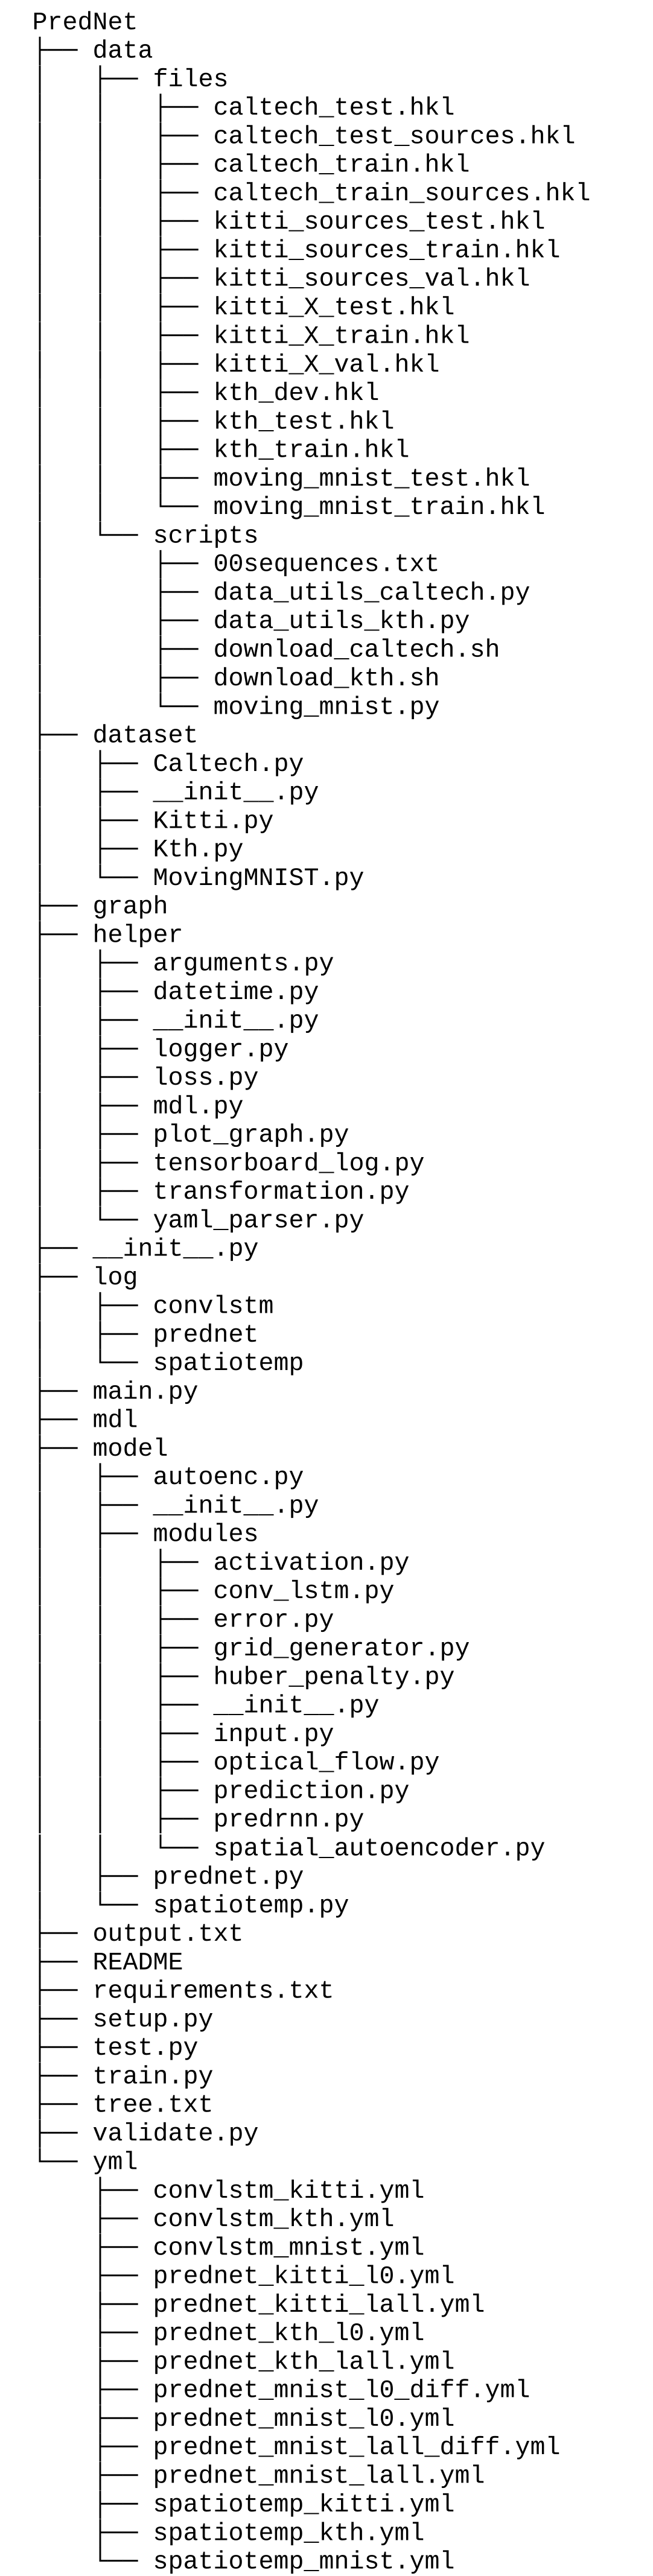
\includegraphics[width=0.35\textwidth]{../Images/tree.png}
   \centering
   \caption{Tree of Implementation}
   \label{fig:tree}
  \end{figure}\noindent
 % subsection
 \subsection*{Code usage}
  \begin{figure}[H]
   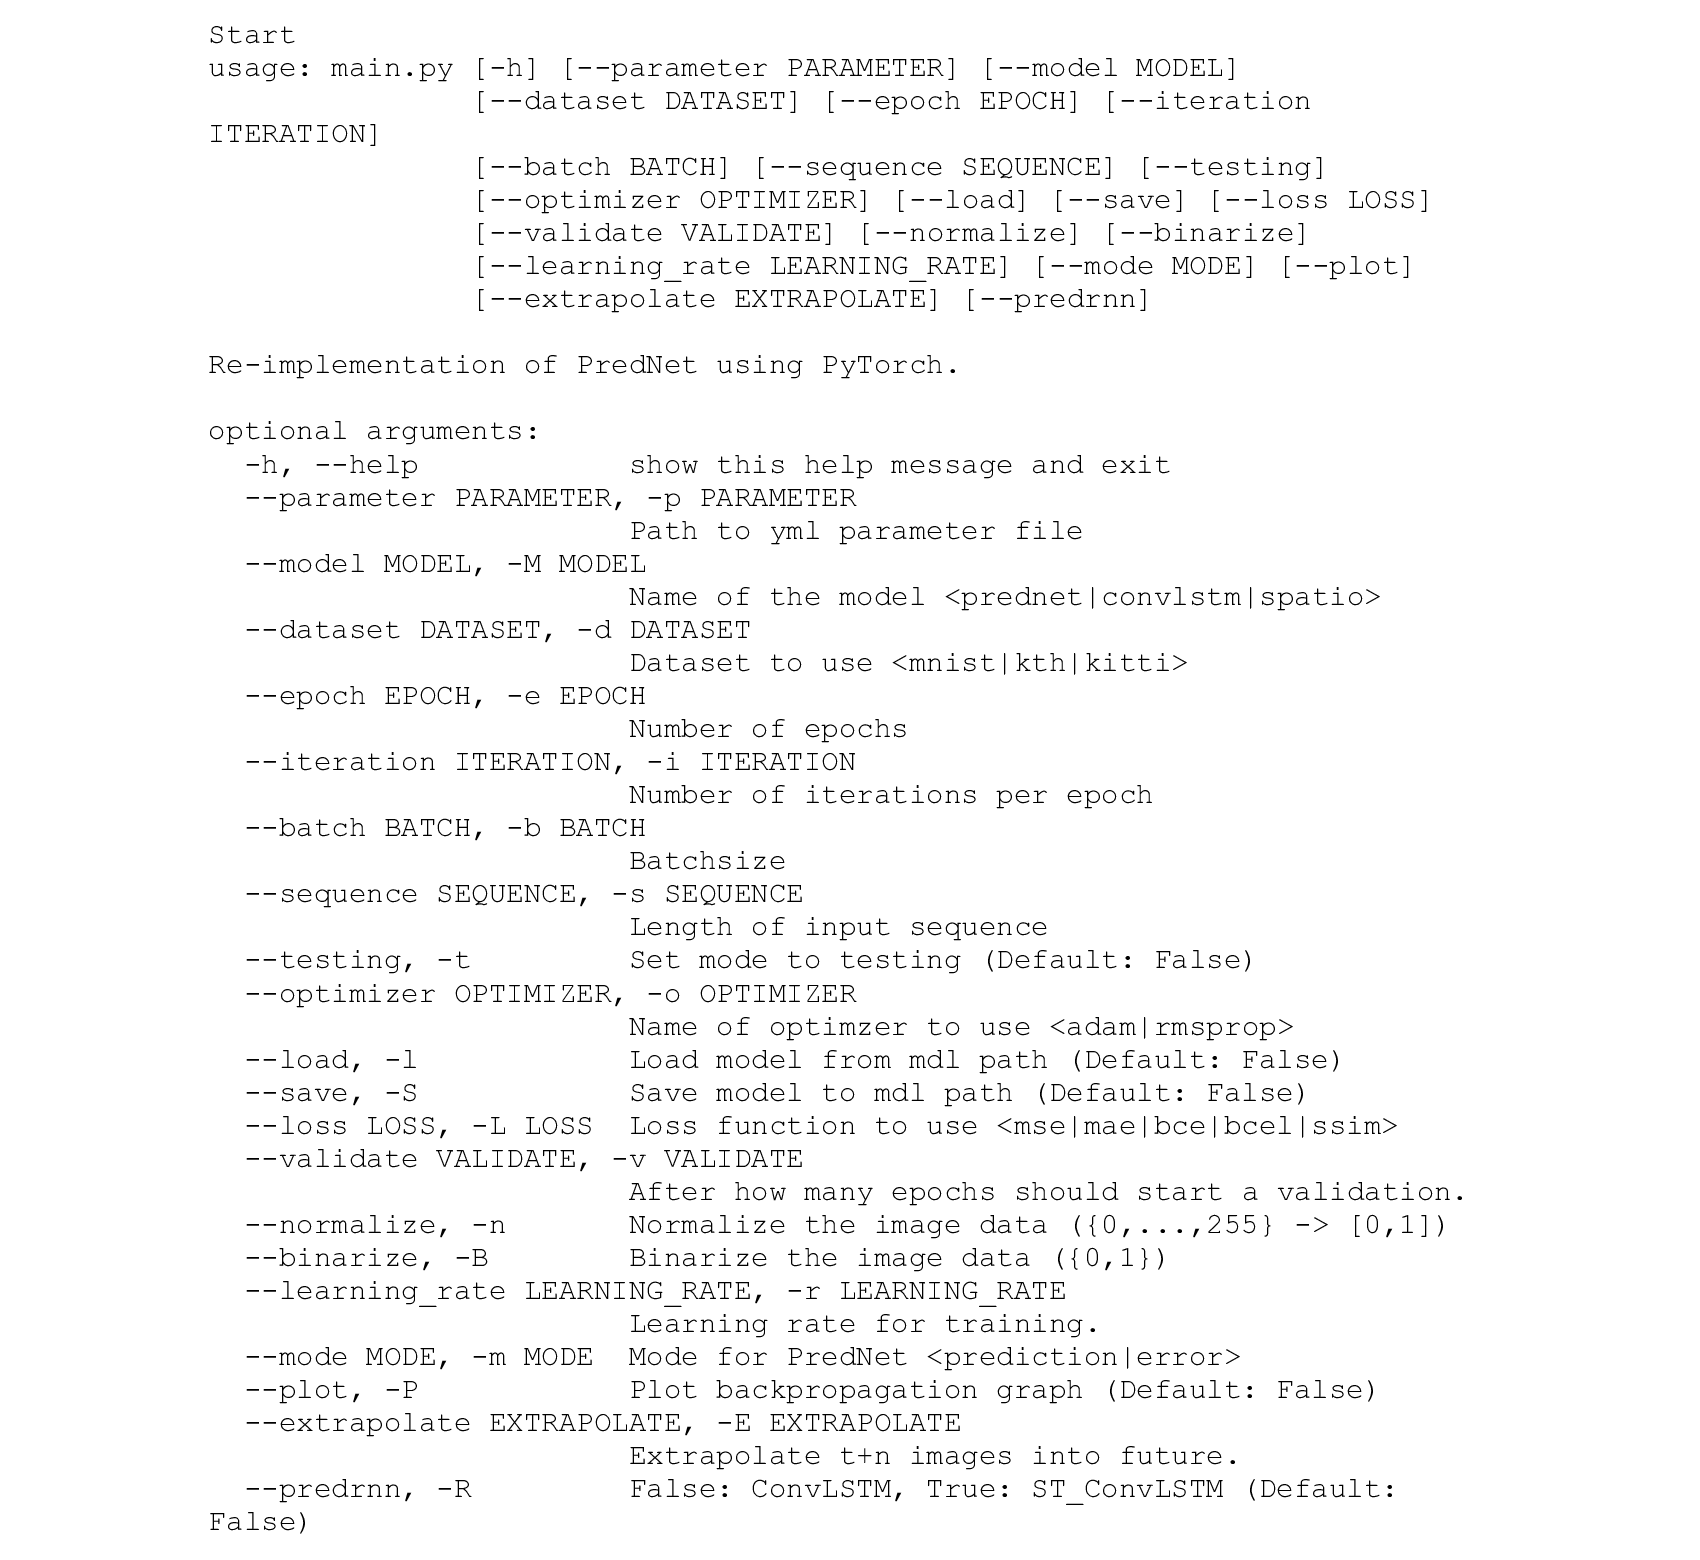
\includegraphics[width=1.0\textwidth]{../Images/usage.png}
   \centering
   \caption{Usage of Implementation}
   \label{fig:tree}
  \end{figure}\noindent
 \newpage 
 % subsection
 \subsection*{Class diagram}
  \begin{figure}[H]
   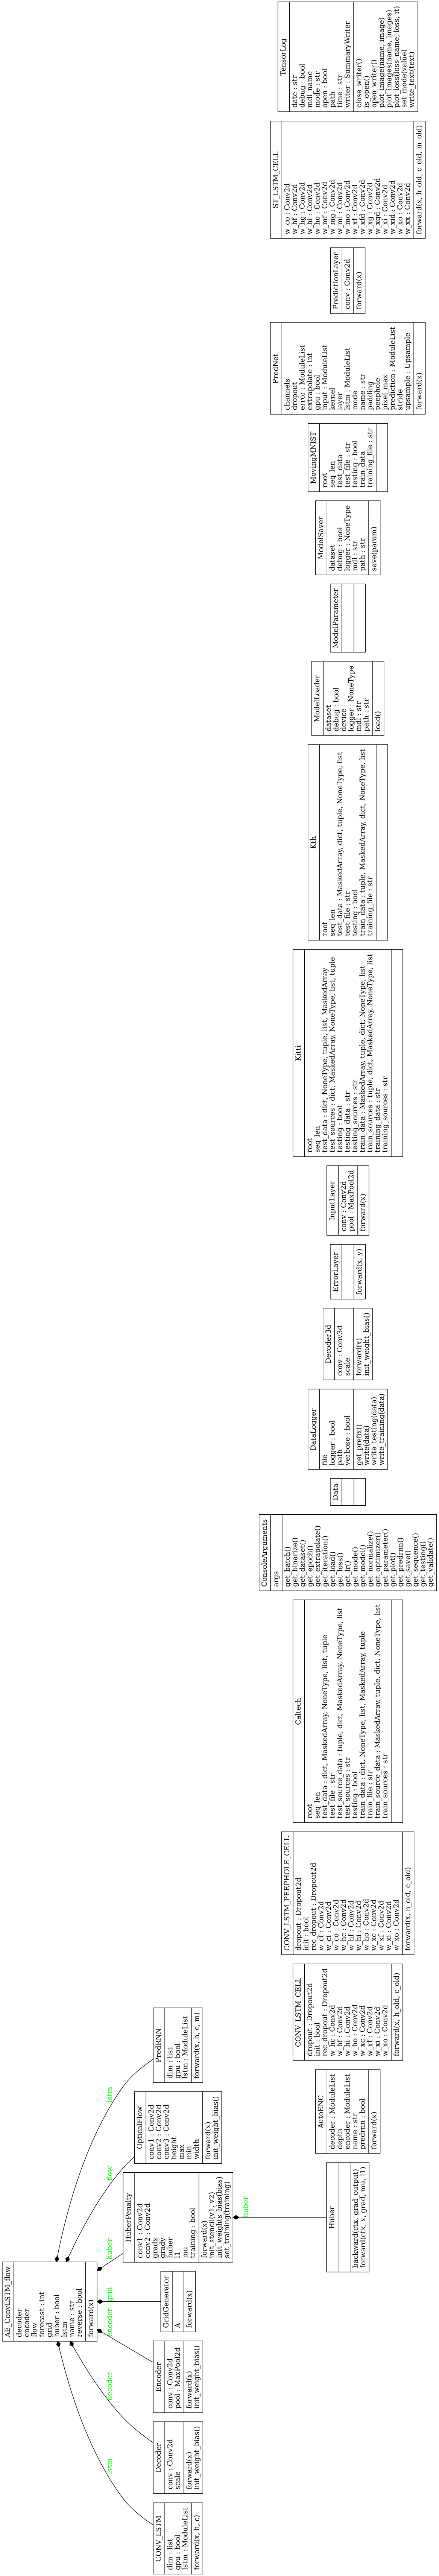
\includegraphics[width=0.23\textwidth]{../Images/classdiagram.png}
   \centering
   \caption{Class diagram, automatically provided by \href{https://pypi.org/project/pyreverse/}{pyreverse}. (pyreverse is not able find connections if loops are 
   used.)}
   \label{fig:tree}
  \end{figure}\noindent
 % subsection
 \subsection*{Package diagram}
  \begin{figure}[H]
   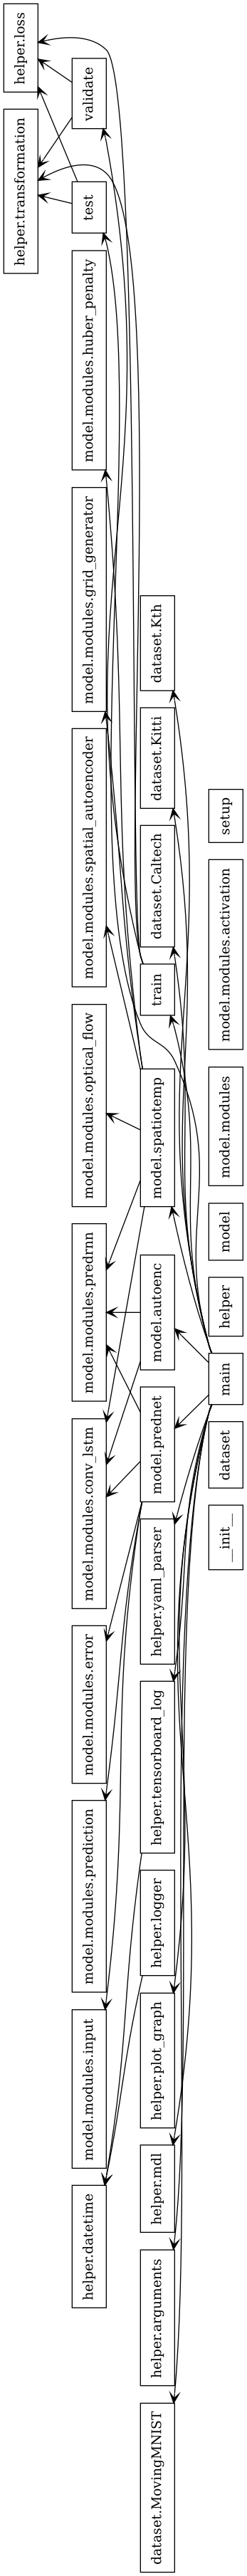
\includegraphics[width=0.13\textwidth]{../Images/packagediagram.png}
   \centering
   \caption{Package diagram, automatically provided by \href{https://pypi.org/project/pyreverse/}{pyreverse}}
   \label{fig:tree}
  \end{figure}\noindent
  
